\chapter{Laser scanning}

Jako Laser scanning se~označuje technologie využívající rychle se~pohybující laserový paprsek. Mezi tradfiční techniky pohybu paprsku spadají akusticko-optické skenery, hranolové skenery a~galvanometrové skenery~\cite{mems-review}.

\section{Akusticko-optické skenery}
Princip Akusticko-optických~(AO) skenerů spočívá ve~změně indexu lomu materiálu optiky, když ním prochází akustická vlna. Tato změna indexu lomu způsobí změnu směru paprsku, který optikou prochází.~\cite{scanning-handbook}

AO skenery se~nejlépe hodí do~systémů s~rozlišením\footnote{Rozlišení laserových skenerů je~počet všech různých pozic, do~kterých je~skener schopen nasměrovat paprsek.} přibližně 1~000 bodů.
Další charakteristikou AO~skenerů je~možnost přenést paprsek na~libovolný bod~v časovém úseku řádově 10~$\mu$s.~\cite{scanning-handbook}

Existuje mnoho systému využívajících AO~skenery, možná nejzajímavější jsou laserové tiskárny, které naplno využívají schopnosti AO~skenerů.~\cite{scanning-handbook}

\section{Hranolové skenery}
Hranolové skenery se~vyznačují rotujícím hranolem se~zrcadlivými stranami (dále \uv{zrcátky}).
Při rotaci hranolu se~mění úhel dopadu laserového paprsku na~zrcátko, a~díky tomu se~mění směr odraženého paprsku, viz~obrázek~\ref{fig:polygon-scanner}~\cite{scanning-handbook}.

\begin{figure}[H]
  \centering
  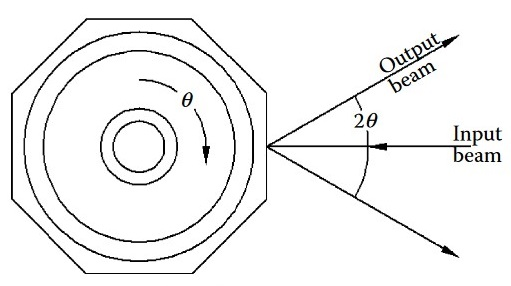
\includegraphics[width=0.5\textwidth]{img/polygon-scanner.jpg}
  \caption{\label{fig:polygon-scanner} Mechanika polygonových skenerů~\cite{scanning-handbook}.}
\end{figure}

% \begin{figure}[htb]
%   \centering
%   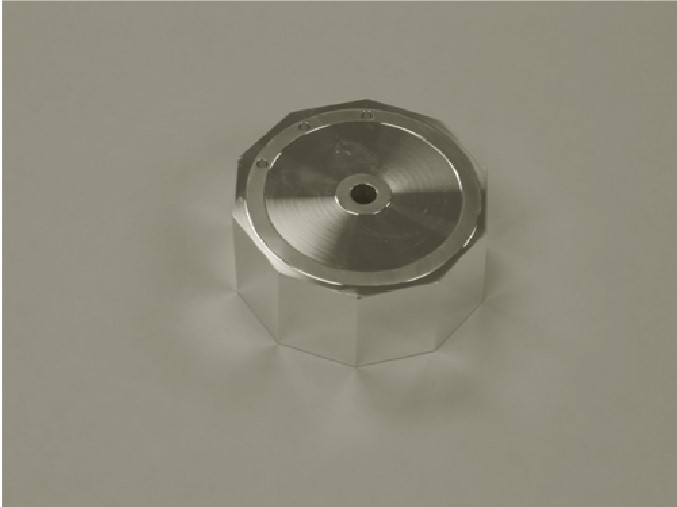
\includegraphics[width=0.5\textwidth]{img/polygon-prismatic-mirror.jpg}
%   \caption{\label{fig:polygon-prismatic-mirror} hranolové zrcátko polygonového skeneru~\cite{scanning-handbook}.}
% \end{figure}

% \begin{figure}[htb]
%   \centering
%   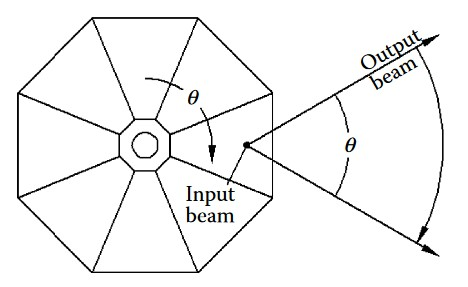
\includegraphics[width=0.5\textwidth]{img/polygon-pyramidal-mirror.jpg}
%   \caption{\label{fig:polygon-pyramidal-mirror} pyramidové zrcátko polygonového skeneru~\cite{scanning-handbook}.}
% \end{figure}
%

S jedním hranolem by~hranolové skenery byly schopny směřovat paprsek pouze v~jedné rovině -- při projekci by~bylo možné vykreslit maximálně čáru. Tuto limitaci lze~kompenzovat přidáním malého rozdílu ve~směřování každé strany hranolu, viz obrázek~\ref{fig:polygon-angular-variation}. S~touto úpravou každá strana hranolu vykreslí jednu svoji přímku lehce posunutou vůči přímkách ostatních stran. Hranol s~\It{n}-úhelníkovou podstavou je~schopen vykreslit \It{n}~přímek.
Další možností je~kombinovat původní pravidelný hranol s~galvanometrem, kdy~galvanometr nastaví jednu souřadnici paprsku a~hranol na~této souřadnici vykreslí přímku.

Tento typ~skeneru se~využívá hlavně pro~senzory skenující na~přímce (např. skenery čárových kódů~\cite{history-of-barcode-scanning}), nebo při rastrovém procházení plochy (například 3D skenování, nebo promítání rastrových obrázků, viz~obrázek~\ref{fig:harddrive-projection}).

\begin{figure}[H]
  \centering
  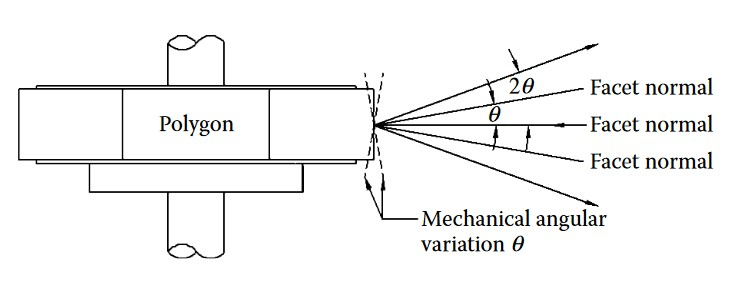
\includegraphics[width=0.8\textwidth]{img/polygon-angular-variation.jpg}
  \caption{\label{fig:polygon-angular-variation} Úhlová rozdílnost zrcátek polygonového skeneru a~paprsky od~nich odražené~\cite{scanning-handbook}.}
\end{figure}


\begin{figure}[H]
  \centering
  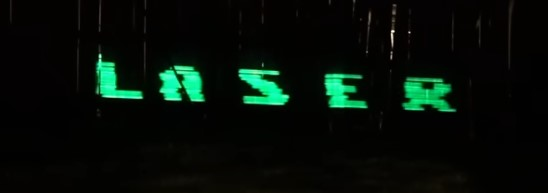
\includegraphics[width=0.5\textwidth]{img/harddrive-projection.jpg}
  \caption{\label{fig:harddrive-projection} Příklad projekce laserového projektoru s~polygonovým skenerem~\cite{harddrive-projector-youtube}}
\end{figure}

\section{Galvanometrové skenery}
V galvanometrových skenerech je~paprsek odrážen dvěma zrcátky připevněnými na~páru galvanometrů. Ty~bývají situovány tak, aby~každý galvanometr ovládal jednu osu~pohybu paprsku, viz~obrázek~\ref{fig:scanner-constructions}.~\cite{scanning-handbook}

Narozdíl od~hranolových skenerů je~s~galvanometrovým skenerem možné zastavit libovolnou osu~pohybu -- vykreslovat čáry orientované jakýmkoliv směrem.

\begin{figure}[htb]
  % \vspace{-0.1\textwidth}
  \centering
  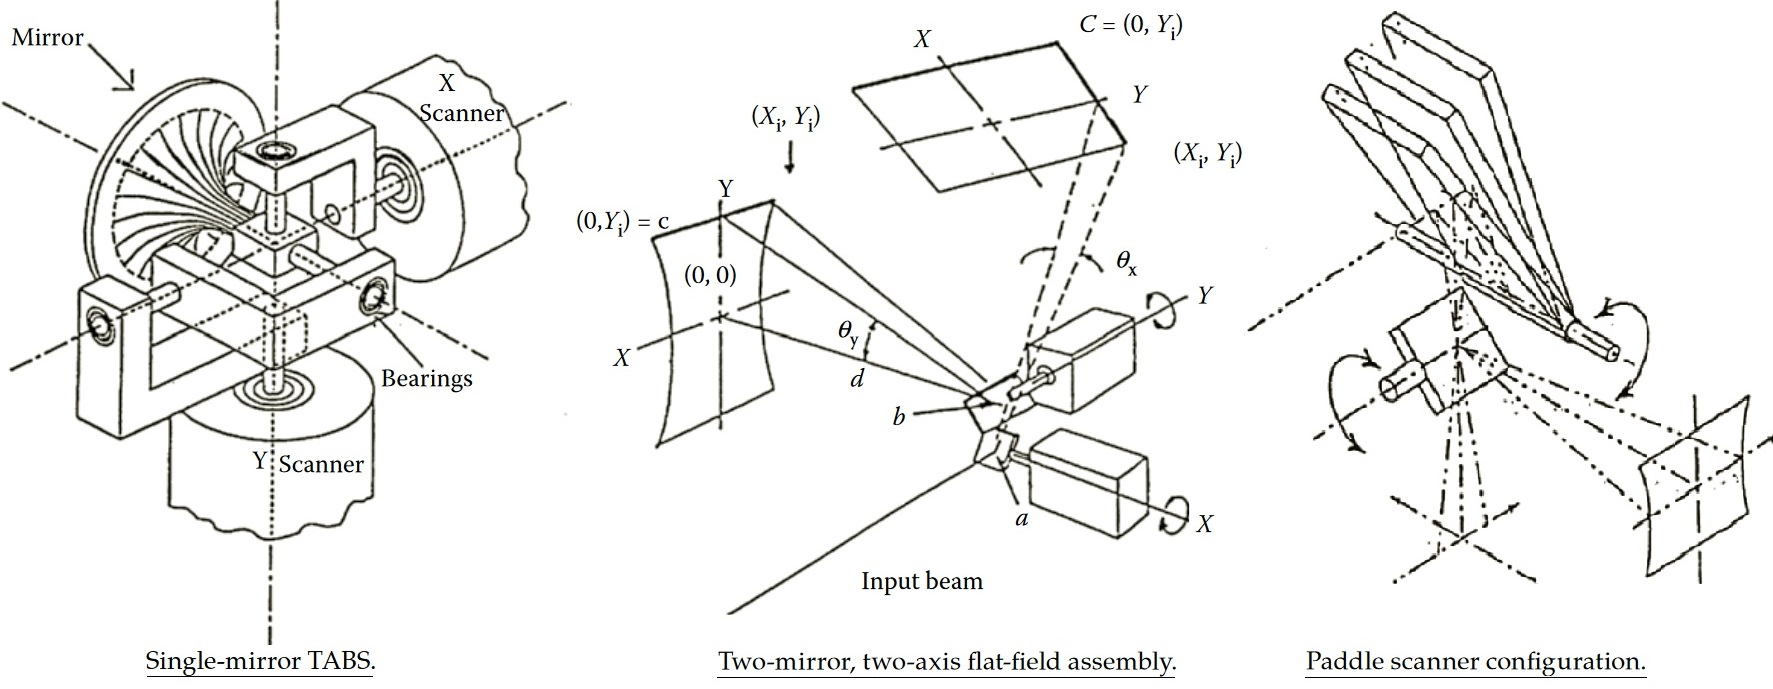
\includegraphics[width=0.5\textwidth]{img/scanner-constructions.jpg}
  \caption{\label{fig:scanner-constructions} Konstrukce galvanometrových skenerů~\cite{scanning-handbook}.}
\end{figure}

\subsection{Galvanometr}
Slovem galvanometr se~označuje přístroj úrčený k~detekci nebo měření velice malého elektrického proudu~\cite{galvo-definition}. Galvanometry při měření využívají interakce magnetického pole trvalého magnetu a~cívky protékané proudem. Tato interakce vychýlí ručičku ukazující na~stupnici, nebo zrcátko odrážející paprsek, který dopadá na~stupnici.~\cite{wiki-galvo}

Můžeme tedy výchylku galvanometru přesně ovládat proudem, který ním protéká.

Galvanometry se~dají rozdělit na~galvanometry bez~zpětné vazby (open-loop) a~se~zpětnou vazbou. K~těm bývají připojeny ovládací obvody, které z~galvanometrů získávají informace o~jejich pohybu a~podle nich regulují signál posílaný do~galvanometrů.~\cite{wiki-galvo}

Dále se~dělí dle~pohyblivé součástky. V~galvanometru je~buď trvalý magnet pevně ukotven a~cívka pohyblivá (moving coil), nebo naopak (moving magnet). % https://prirucka.ujc.cas.cz/?id=151#nadpis3

Dnes se~v~kontextu laserových skenerů prakticky vždy používají galvanometry s~pohyblivým magnetem a~se~zpětnou vazbou. Ta~je~zajištěna čtením z~variabilního kondenzátoru umístěného v~galvanometru.

\begin{figure}[htb]
  \centering
  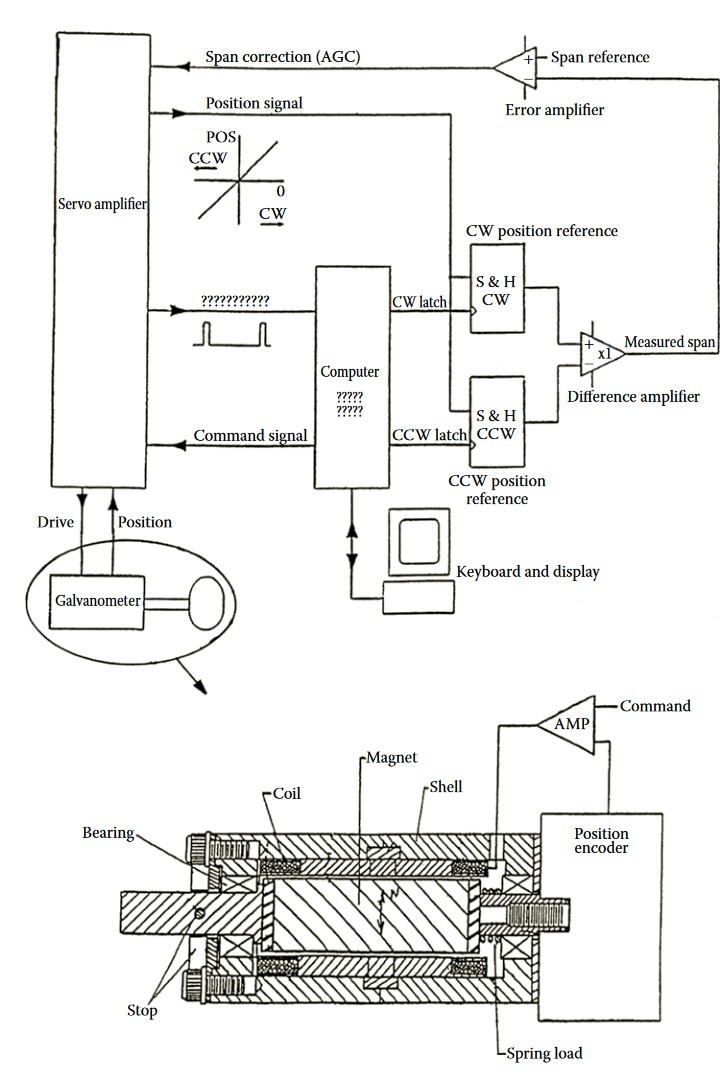
\includegraphics[width=1\textwidth]{img/galvanometer-detail.jpg}
  \caption{\label{fig:galvanometer-detail} Zapojení a~vnitřní konstrukce galvanometrů~\cite{scanning-handbook}.}
\end{figure}
